\section{Participants}
A total amount of \todo{number} participants were recruited from \todo{campus/friends/etc}. They were divided into a human trainer (HTG) and interactive system group (ISG), each with \todo{number} participants. Among them \todo{X} were males and \todo{X females}. The age ranged from \todo{min age} to \todo{max range} (\todo{mean, avg, SD}), the body height from \todo{min height} to \todo{max height} (\todo{mean, avg, SD}), and the weight from from \todo{min weight} to \todo{max weight} (\todo{mean, avg, SD}). All participant agreed to train without shoes but with socks to provide a consistent training condition per participant.
\todo{X} participants had prior experience with an interactive device whereas \todo{X} participants had few experience and \todo{X} had no experience. Regarding slacklining some stood either one up to three times on a slackline or never. All participants had no contact with a slackline in the last two years. No participant had experienced prior knowledge in balance activities. The physical activity level in their job and spare time as well as sport activity, ranged from very low active up to highly active (Table \todo{table}). All participants were briefed and gave their consent for taking part on the study and agreed with audiovisual data recording. The present study was approved by the local ethic commission. 
%At last she had to agree for participating the study and confirm to be recorded via audio and video for later analysis.

\begin{figure}[htb]
	\centering
	\begin{minipage}[t]{1\linewidth}
		\centering
		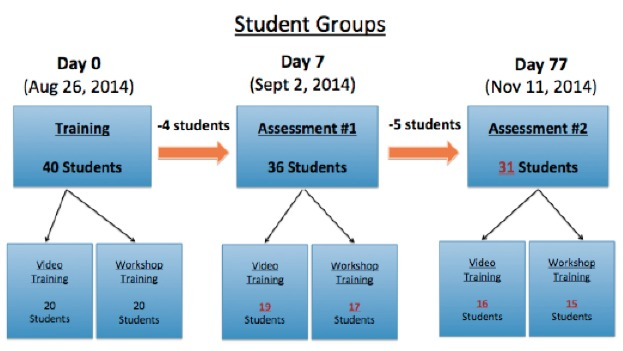
\includegraphics[width=0.8\linewidth]{Pictures/6_studyGroupsExample}
		\caption{Study groups example}
		\label{fig:6_studyGroups}
	\end{minipage}
\end{figure}